%Aditya Tatwawadi John Locke report Summer 2021
\documentclass[a4paper,12pt]{article}

    %Everything in the general pre-amble:

    % Basic figure setup, for now with no caption control since it's done
    % automatically by Pandoc (which extracts ![](path) syntax from Markdown).
    \usepackage{graphicx}%to upload graphics
    % Maintain compatibility with old templates. Remove in nbconvert 6.0
    \let\Oldincludegraphics\includegraphics
    \usepackage{setspace}
    \usepackage{caption}
    \usepackage{subcaption}
    \usepackage[sorting = none]{biblatex}
    \addbibresource{johnlocke.bib}
    \graphicspath{/Users/adityatatwawadi/Desktop/Projects/Python/JohnLocke2021/LaTeX - JL/JohnLocke Images}
    \usepackage[colorlinks, citecolor = blue, urlcolor = blue]{hyperref}
    \usepackage{float}
    \usepackage{color} 
    \floatplacement{figure}{H} % forces figures to be placed at the correct location
    \usepackage{xcolor} % Allow colors to be defined
    \usepackage{enumerate} % Needed for markdown enumerations to work
    \usepackage[margin = 1in]{geometry} % Used to adjust the document margins
    \usepackage{amsmath} % Equations
    \usepackage{amssymb} % Equations
    \usepackage{textcomp} % defines textquotesingle
    % Hack from http://tex.stackexchange.com/a/47451/13684:
    \AtBeginDocument{%
        \def\PYZsq{\textquotesingle}% Upright quotes in Pygmentized code
    }
    \usepackage{listings}%to upload python code
    \usepackage{upquote} % Upright quotes for verbatim code
    \usepackage{eurosym} % defines \euro
    %    \usepackage[mathletters]{ucs} % Extended unicode (utf-8) support
    \usepackage{fancyvrb} % verbatim replacement that allows latex
    \usepackage{grffile} % extends the file name processing of package graphics
    \renewcommand{\lstlistlistingname}{List of Python Code:}
    \hypersetup{colorlinks=true,linkcolor=black}

    %Style of code to make it readable
    \lstdefinestyle{chstyle}{%
    backgroundcolor = \color{gray!12},
    basicstyle = \ttfamily\small,
    commentstyle = \itshape\color{black},
    keywordstyle = \bfseries\color{green!40!black},
    stringstyle = \color{red},
    identifierstyle=\color{blue},
    showstringspaces = false,
    numbers = left,
    numberstyle = \footnotesize\color{gray},
    numbersep = 10pt,
    stepnumber = 1,
    tabsize = 2,
    frame = TBLR,
    framerule = 1pt,
    rulecolor = \color{black},
    breaklines = true,
    inputpath = johnlockecode
    }

\author{Aditya Tatwawadi}
\title{Audio Signal Processing}
\date{August 2021}

%Title Page
\begin{document}
    \begin{titlepage}
        \begin{center}
            \vspace*{1cm}
    
            \LARGE
            \textsc{\textbf{An Insight into Audio Signal Processing for Musical Information Retrieval}}
    
            \vspace{0.5cm}
                
            \textit{Aditya Tatwawadi - Wren's}
                
            \vspace{4cm}
            \LARGE
            
\includegraphics[width=0.4\textwidth]{westminsterschool}
            
            \Large
            \textsc{\textbf{
            Westminster School\\
            Computational Engineering Project\\
            John Locke\\
            August 2021}}
                
        \end{center}
    \end{titlepage}

    %General formatting
    \pagenumbering{roman}
    \pagenumbering{arabic}  

    %Table of Contents
    \doublespacing
    \normalsize
    \tableofcontents
    \begin{center}\rule{0.9\linewidth}{0.5pt}\end{center}
    \lstlistoflistings 
    \singlespacing
    \normalsize
     
    %Foreword
    \textbf{Foreword:} 
    \vspace{0.2cm}
    \newline
    My main goal of this John Locke has been to make an application with Python. Please reach out if you would like a live demonstration. Much of this report is supplentary as an overview of Audio Signal Processing. I also have very little to no background in music.
    \newline
    \href{https://github.com/aditya-tatwawadi/Audio-Signal-Processing}{Consider accessing GitHub repository here \parencite{GitHubRepo}}
    \newpage
    
\begin{center}
\Large
\textbf{An Insight into Audio Signal Processing}
\end{center}

\begin{center}\rule{0.9\linewidth}{0.5pt}\end{center}

%Introduction
\normalsize
\section{Introduction}
\textbf{Audio Signal Processing (ASP)} has addressed many problems previously faced across various industries. Being able to identify songs was one such notoriously difficult issue.
Companies such as \textit{Shazam} have found ingenious methods to solve this and create a user-friendly product. Today, \textit{Shazam} is valued at over \$400 million,
and has been acquired by \textit{Apple} \parencite{BBCvaluation}. Modern day applications of ASP include data-compression, speech processing, noise-cancellation and more.
This is an industry to look out for.

\begin{figure}[h!]
    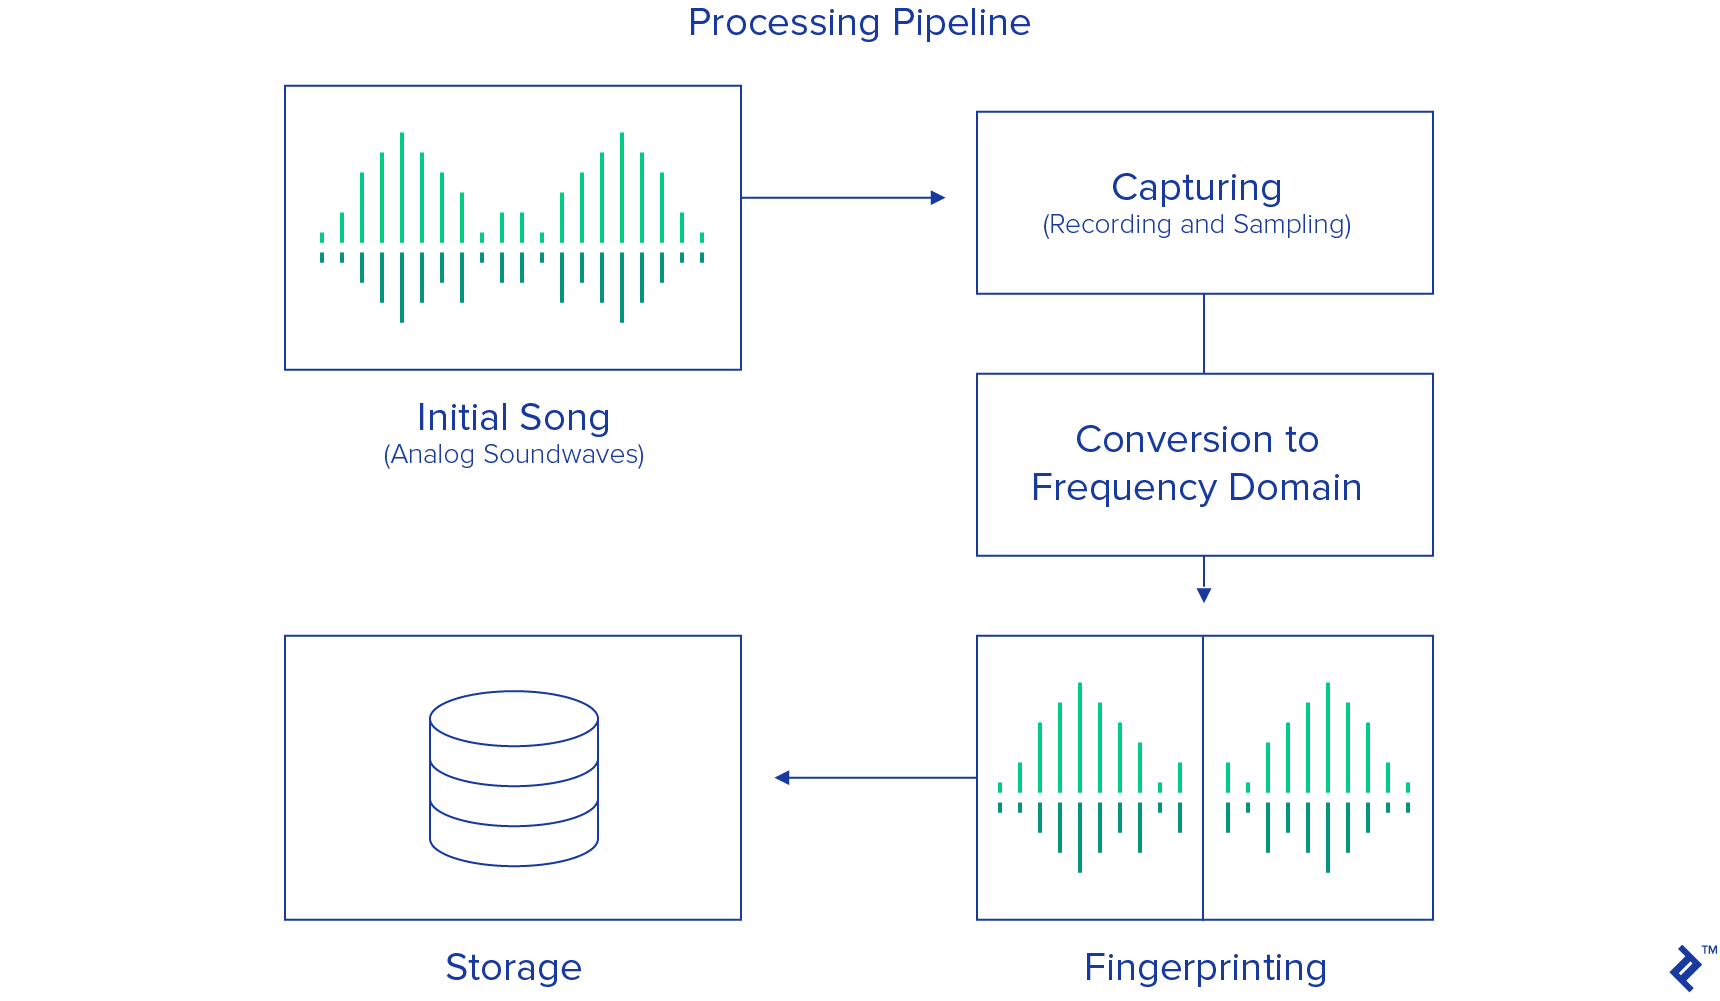
\includegraphics[width=16cm]{shazamdemo.png}
    \centering
    \caption{Shazam application timeline \parencite{ShazamASP}}
    \end{figure}

The theory and applications behind ASP have historically been championed at \textit{Bell Labs}
since the start of the 20th century after the introduction of telephones, radios and phonographs. 
Previously, analogue signals - which relied on continuous signals being "analogous" to the sound waves in air - needed to be
physically altered by electric circuits. This made the process cumbersome and cost inefficient. Thanks to the advent of computational power, digital signals can now be used to express
audioforms in binary numbers. This makes modern day signal processing more powerful, reliable and cheaper to implement \parencite{Udo1997}.
\newline

In this report, the focus will be placed on music information retrieval, as well as the insights into the mathematics and physics to achieve this. Additionally, I have also built
my own application to give song predictions using the \textit{Python 3} programming language. This can be found referring to section
\ref{sec2} on page \pageref{sec2}.

\newpage

%Parson's code
\normalsize
\section{The Parson's Code}

\subsection{Theory}
\label{sec1}    
Developed by Denys Parsons in his 1975 book \textit{The Directory of Tunes and Musical Themes}, the Parson's code is a surprisingly simple yet accurate way of identifying melodies; this makes it well-suited towards 
music information retrieval \parencite{ParsonsCodeDOTMT}.
\newline

One of the key benefits of using the Parson's code is that no technical music knowledge is needed to implement it. It works through melodic motion: that is by identifying movements of pitch varying up and down. The first tone of reference is denoted with an asterix: *. If the following note
is higher, a U (up) is used. If the following note is lower a D (down) is used. If the following note is repeated, a "R" (repeat) is used.
\newline

e.g. The Parson's code to display \textit{Fur Elise} would be:
\newline 

*DUDUDUDDDUUU.

\vspace{0.3cm}
\begin{figure}[h!]
    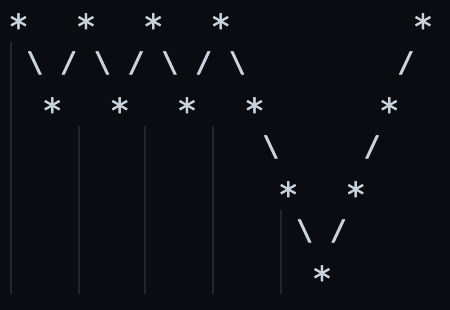
\includegraphics[width=10.2cm]{furelisecode.png}
    \centering
    \caption{Parson's contour for "Fur Elise" using my application}
    \end{figure}

The Parson's code is only reliable in music retrieval if there is an identifiable, 
but not simultaneously varied pitch. Due to this, extraction is only feasible for classical/ folk/ distinct melodies, and not so much for hip-hop/ jazz
songs or anything containing mixed timbres. Other limitations include difficulty in storing data, due to the Parson's code being relatively unknown and not well documented.

\subsection{Practical Implementation of Parson's Code}
\label{sec2}
On page \pageref{Appendix} is the code of my project written to suggest to a user the top 3 most likely song predictions of a given MIDI audio file. See Listings 1,2,3 from Appendix.
To access a cleaner version of my code, consider forking my repository on \textit{Github} \parencite{GitHubRepo}. An explanation can be found on page \pageref{explanationofcode}.

\newpage
\subsection{Brief Overview of Application}
\label{explanationofcode}

\begin{figure}[h!]
    \centerline{%
    
\includegraphics[width =2.5cm]{PythonLogo.png}
    
\includegraphics[width = 2.5cm]{GithubLogo.png}
    }%
\end{figure}

%\lstinputlisting[language = Python, style = chstyle, caption = main.py]{main.py}
%\lstinputlisting[language = Python, style = chstyle, caption = compute.py]{compute.py}
%\lstinputlisting[language = Python, style = chstyle, caption = webscrape.py]{webscrape.py}

There are 3 main files which run the code - main.py, compute.py and webscrape.py. 

\begin{itemize}

    \item The main.py file imports the code from the other two files, and produces an image from 
    \textit{Musipedia}: which has the information about the top 3 most likely song names and their composer.

    \item The compute.py file is an algorithm to extract the Parson's code from a MIDI file, produce a
    visual contour, and store it as a string to be accessed later.

    \item The webscrape.py file hits the internet and uses the \textit{Musipedia} database to extract
    the songs corresponding to the identfied Parson's Code.

\end{itemize}

\begin{figure}[h!]
    \centering
    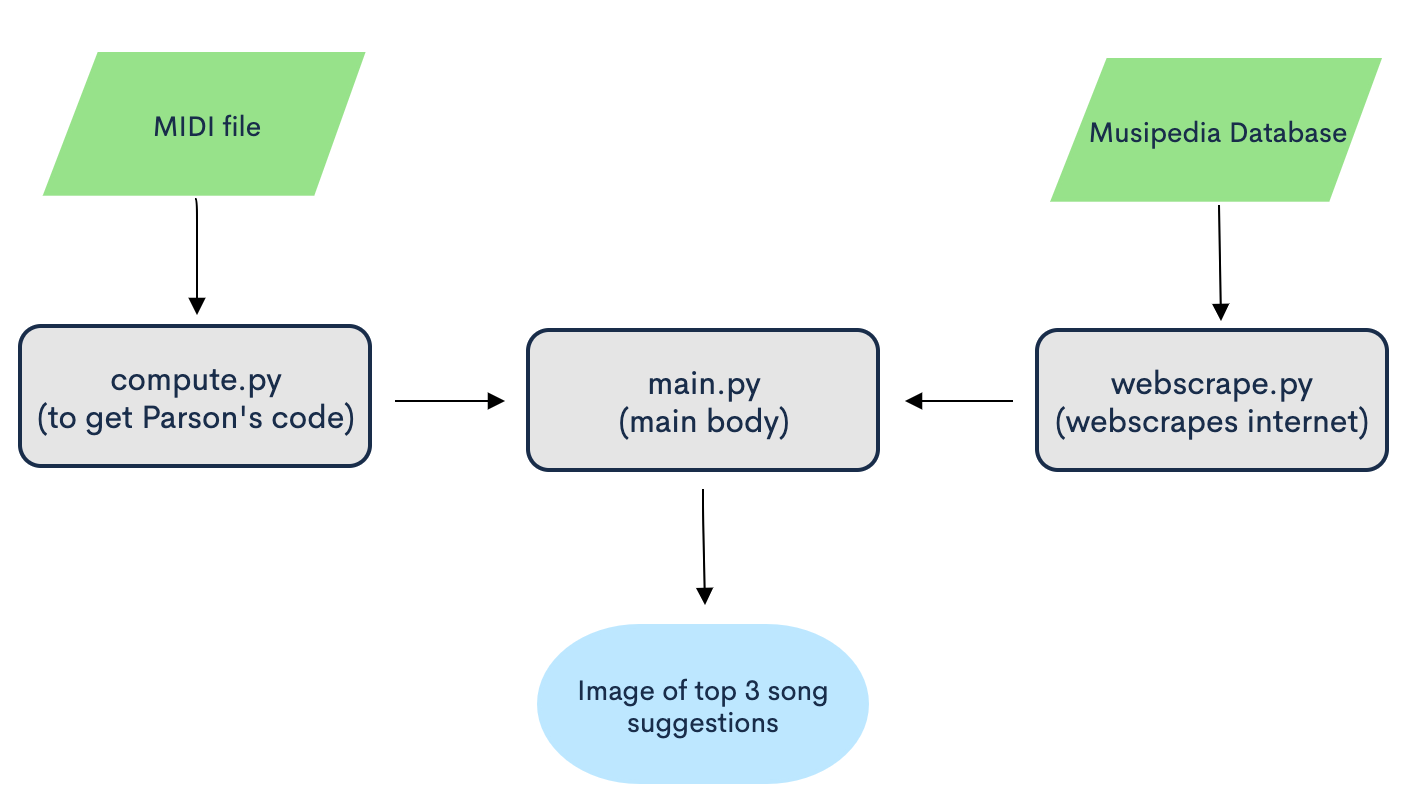
\includegraphics[width=17cm]{flowchart.png}
    \caption{Flowchart of events}
\end{figure}

It is important to note that this is a somewhat abstraction of what is actually happening -
the true computation lies in the \textit{Mido} python library. The MidiFile object is able to read, write and
play back any MIDI files. Although humans cannot hear .mid files like they would a .wav file, midi files are more accurate
in transferring information between different places. 

The next section will consider some of the mathematics and physics behing how exactly an audio file is decomposed, and an insight into 
how more sophisticated methods are used to generalize audio extraction to any type of music.

\newpage
%Scientific methods
\section{Scientific Methods}
\subsection{Physics behind ASP}
\textbf{What is sound?} Sound can be described as a vibration of pressure that propagates as longitudinal waves.
After hitting the eardrum, the vibration is then transmitted to hair cells in the cochlea, which produce electrical signals
to the brain.
\newline

This process of converting to an electrical signal from the pressure of a sound wave (continuous signals) is imitated by recording devices.
In a microphone, the Operational Amplifer (Op-Amp) translates this into an analog voltage signal.
For the continuous signal to be of use, it must be translated into a discrete signal that can be stored digitally. 
This is done by capturing a digital value that represents the amplitude of the signal. 
The quantization of the input means that an analog-to-digital converter performs many conversions on very small pieces of the signal is a process known as sampling \parencite{AdvancePhysicsTextBook}.

\begin{figure}[h!]
    \centering
    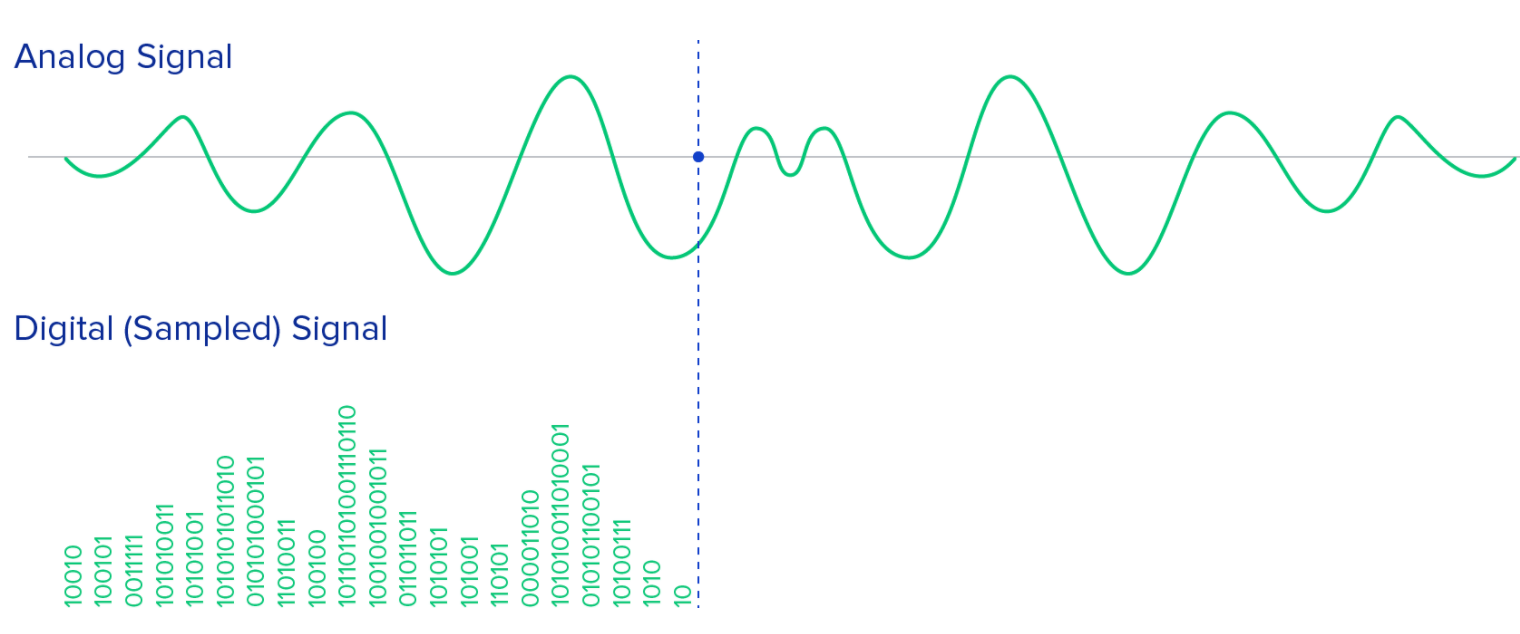
\includegraphics[width=10.5 cm]{analoguetodigital.png}
    \caption{Change of signals \parencite{ShazamASP}}
\end{figure}

Every sound in the world can be represented as the sum of multiples of pure tones in different amplitudes.
As tones are expressed in sinusoidal forms, every sound in the world can therefore be expressed in terms of sinusoidal waves.
Music is played by various instruments and singers, producing a combination of sinewaves at varying frequencies, creating an overall
more obscure sine wave. This can be visualized using a Spectrogram: a 3D graph. Time on the horizontal X axis. Frequency on the vertical Y axis.
A colour representing the amplitude of a defined frequency (in decibels, dB) as the 3rd dimension. Spectrograms can be computed using Fourier Transforms \parencite{ThinkDSP}.

\begin{figure}[h!]
    \centering
    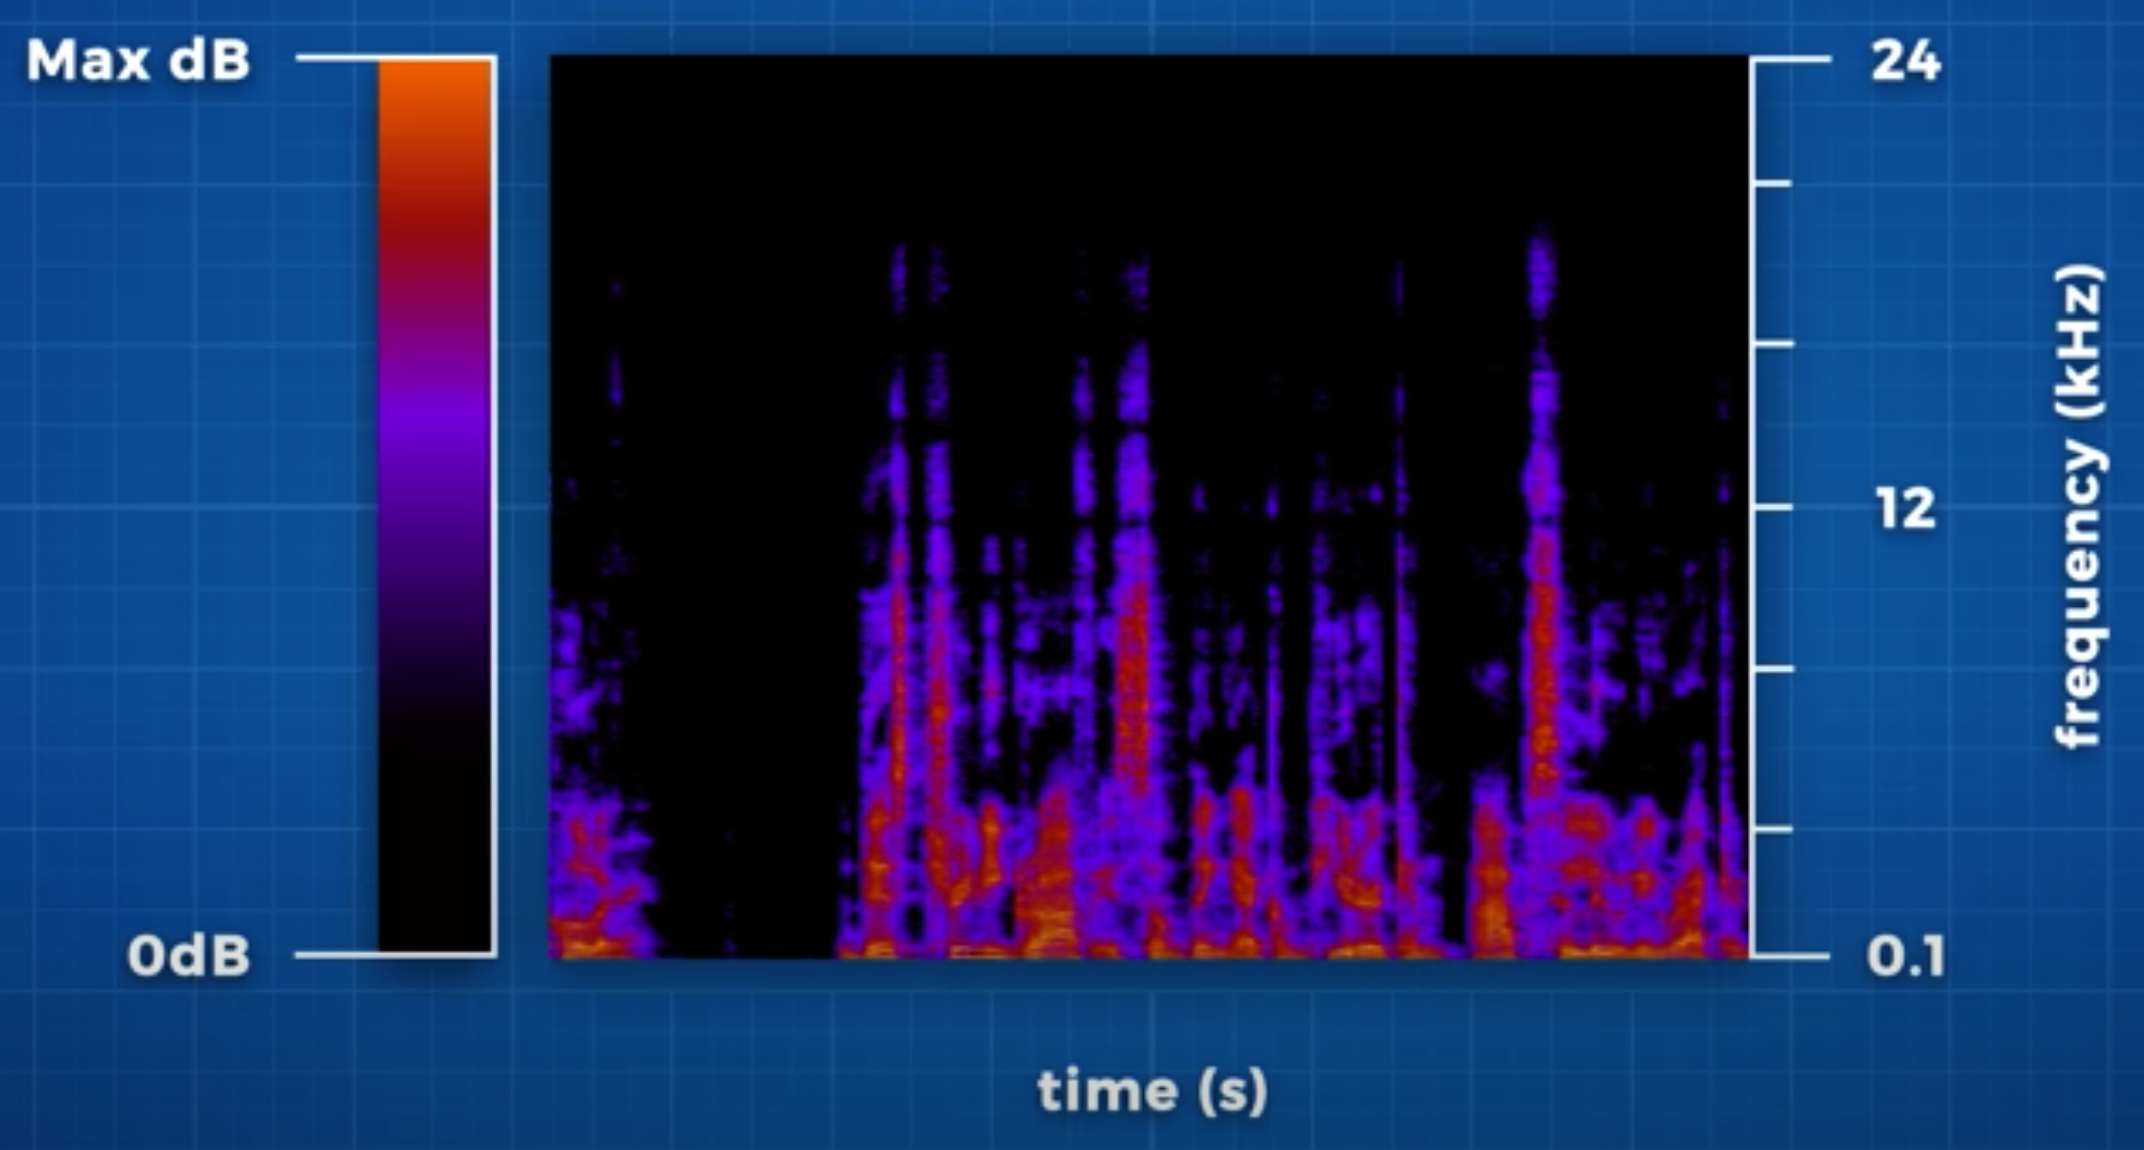
\includegraphics[width=9.5cm]{spectrogram.png}
    \caption{Spectrogram \parencite{RealEngineeringYT}}
\end{figure}

\newpage
\subsection{Mathematics behind ASP}
Sound is made up of a lot of complex wavefunctions. One analogy which could be used to represent the essence of ASP is like blending up a smoothie, and then
trying to reverse-engineering the process to get back its original ingredients. 
\newline

Though of course impossible in real life, in the 19th century Jean-Baptiste Joseph Fourier made a trailblazing advancement that the time domain can be represented
as the sum of multiple sinusoidal signals (as aformentioned on page 5). This is known as the Fourier Series.
\newline

The Fourier Series is used to represent a periodic function by a discrete sum of complex exponentials, while the Fourier transform is then used to represent a general,
non-periodic function by an integral of complex exponentials. The Fourier Transform can be viewed as the limit of the Fourier series of a function as the period approaches infinity, so the limits of integration are $(-\infty, \infty)$.
Instead of trying to crudely fit a signal to model a wave as $A\sin(2\pi(ft + \phi))$, any complex wavefunction can be represeted as the sum of sines and cosines \parencite{3Blue1Brown}. It is important to note that this is one of the most elegant, yet conceptually difficult mathematical topics to understand,
and so cannot be given full justice in just one section of a report. We are concerned with Discrete FT in ASP.

\noindent The Fourier Transform (FT) applies to continuous time giving a continuous spectrum:
\LARGE
\[ \hat{\mathcal{F}}(\xi) = \int_{-\infty}^{+\infty} f(t)e^{-2  \pi  i \xi t} \,dt = \int_{-\infty}^{+\infty} f(x)e^{-i \omega t} \,dt \] \normalsize where $\omega \in (-\infty, +\infty)$ 

\noindent The Discrete Fourier Transform (DFT) applies to finite time giving a discrete spectrum:
\LARGE
\[ X(k) =\sum_{n=0}^{N-1} x(n)e^{-i(2 \pi k n/  N)} \] \normalsize where $n = 0, 1, ..., N-1$ \newline

N is the number of samples that composed the signal.
X(K) represents the kth bit of frequencies.
x(n) is the nth sample of the audio sample.

The use of the complex number $i = \sqrt{-1}$ is purely graphical: the algebra tends to be nicer with geometrically related problems to do with winding or rotation. This can be 
visualized on the Argand Diagram; instead of x,y axis on the Cartesian Plane, there are real and imaginary axis. As the Fourier Transform pertains to circular paths, Euler's Formula is
a suitable way to generate one:

\LARGE
\[ e^{i\theta} = \cos(\theta) + i\sin(\theta)\]

\newpage
\normalsize
In industry, applications like \textit{Shazam} need to optimise processing time to compute a spectrogram, and produce a match to the recorded audio, all within the constraints of the phone's
processor. For this reason, the Fast Fourier Transform (FFT) - which serves the same function as the DFT, but only much faster, - is used. The simplest and most efficient version of the FFT (also used in the numpy package in the implementation of my code in page \pageref{FTimplementation})
is the Cooley-Tukey algorithm. The FFT has a time-complexity of $O(nlog(n))$ which is far superior to DFT's $O(n^2)$ \parencite{CooleyTukey}:

\begin{figure}[h!]
    \centering
    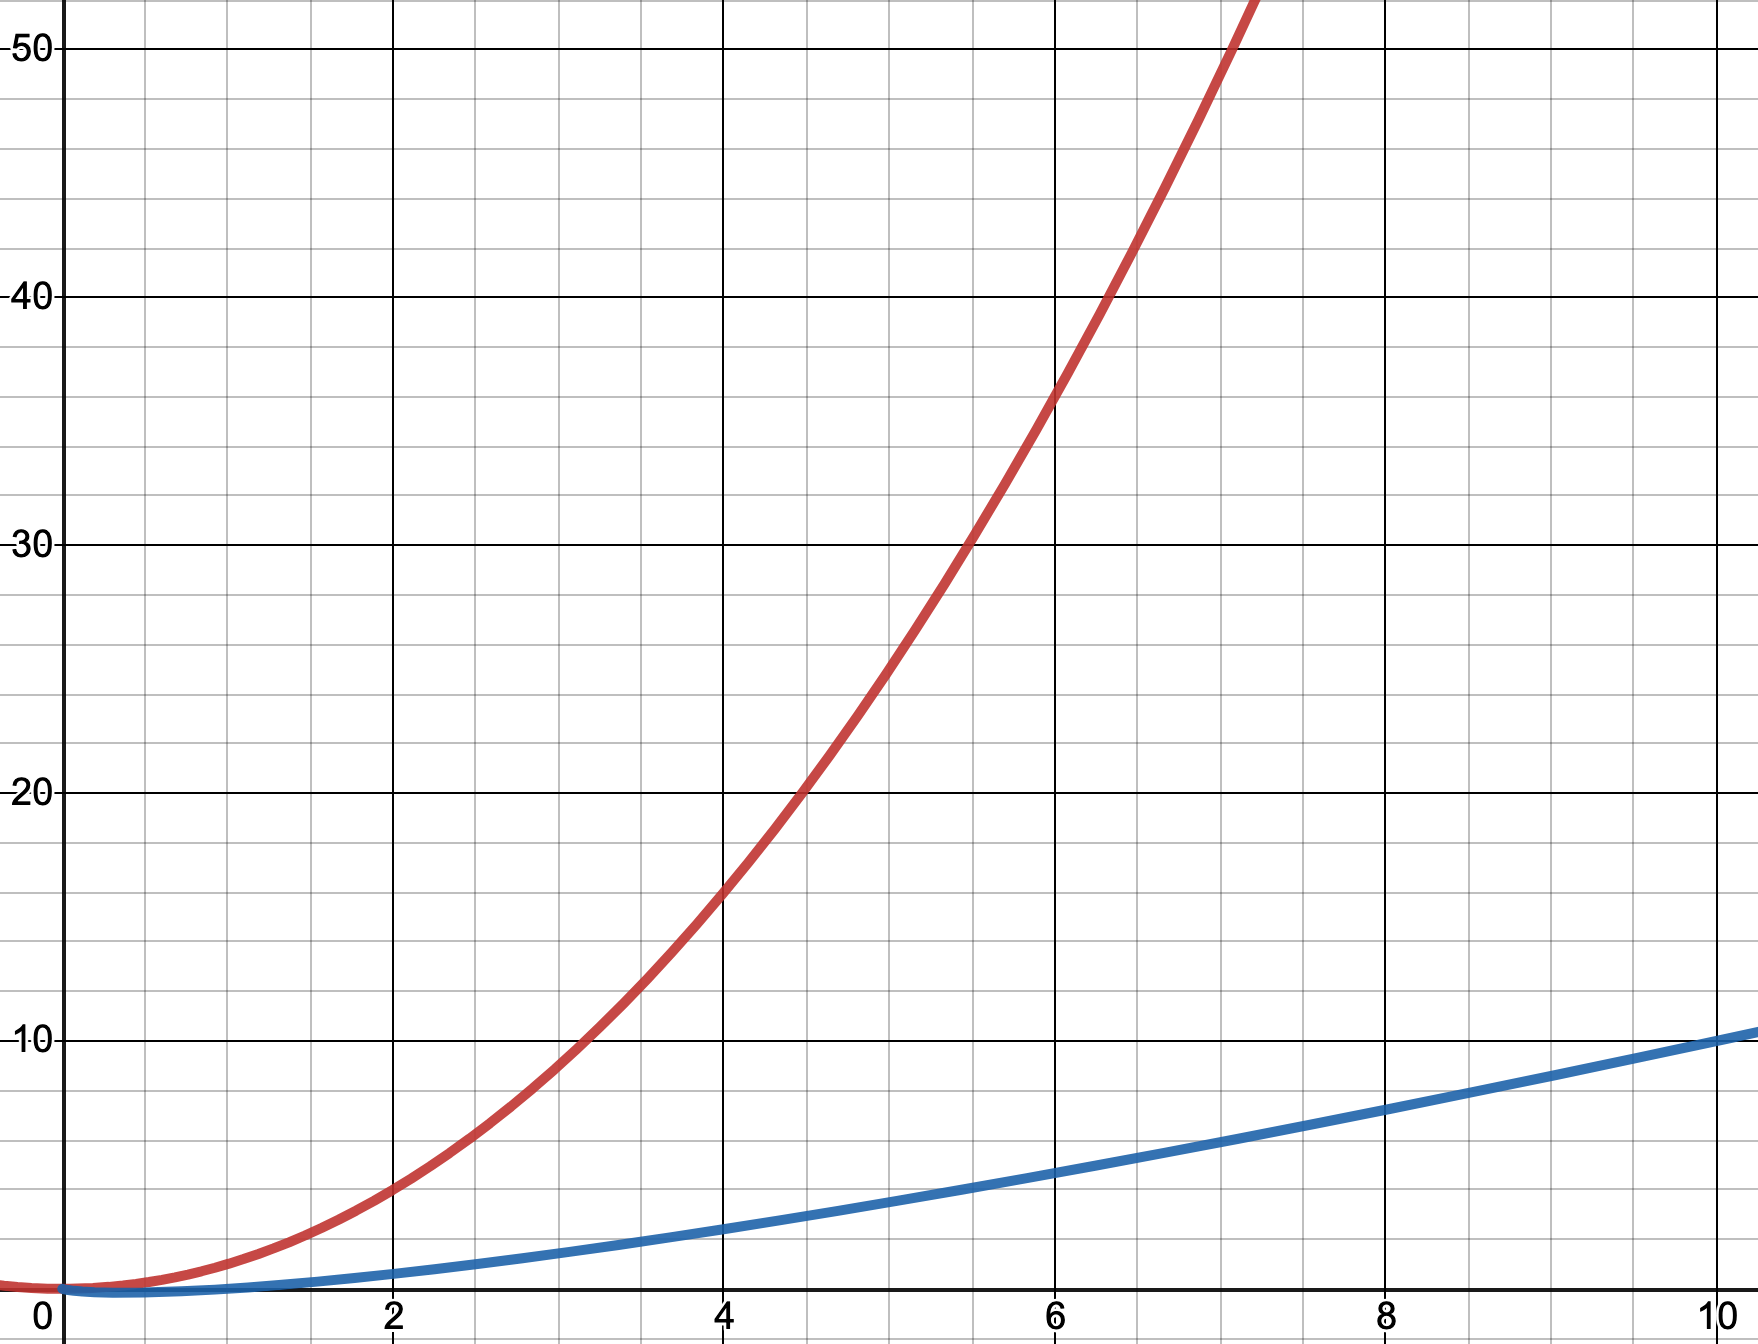
\includegraphics[width=9.5cm]{big0 dft vs fft.png}
    \caption{DFT - Red - $O(n^2)$ || FFT - Blue - $O(nlog(n))$}        
\end{figure}

Such is the importance of the FFT, that the Institue of Electrical \& Electronics Engineers (IEEE)  deemed it as "the most ubiquitous algorithm
in use to analyze digital data", and has been heralded as the top 10 most
influential algorithms of the century by countless publishers and universities \parencite{AlgorithmQuoteft}.

\subsection{Practical Implementation of Fourier Transform}
\label{FTimplementation}

Python Code which performs an FFT can be located in the Appendix under Listing 4 on page 13. This takes a time domain signal, applies a FFT and converts it into a frequency domain signal. Like my previous application, this can be found on my GitHub repository.

\subsection{Database}
As a sidenote, it is intriguing to consider how \textit{Shazam} stores this data. For each individual song, after the FFT is applied and a spectrogram in computed, a \textit{fingerprint} - i.e. a starmap is used to reduce the data
from 3D to 2D. Hash functions and tables are then used in searching algorithms. This goes beyind the scope of this report, but more detail can be located in this article by the founder of Shazam - Avery Wang \parencite{AveryWang}.

%Appendix
\section{Appendix}
\label{Appendix}
A compilation of all code. Everything hosted on GitHub \parencite{GitHubRepo}.
\newpage

%Some alternate set-up
%\newpage
%\lstinputlisting[language = Python, style = chstyle, caption = Fourier Transform Demonstration]{FourierTransformDemo.py}

%\begin{figure}[h!]
%    \centering
%    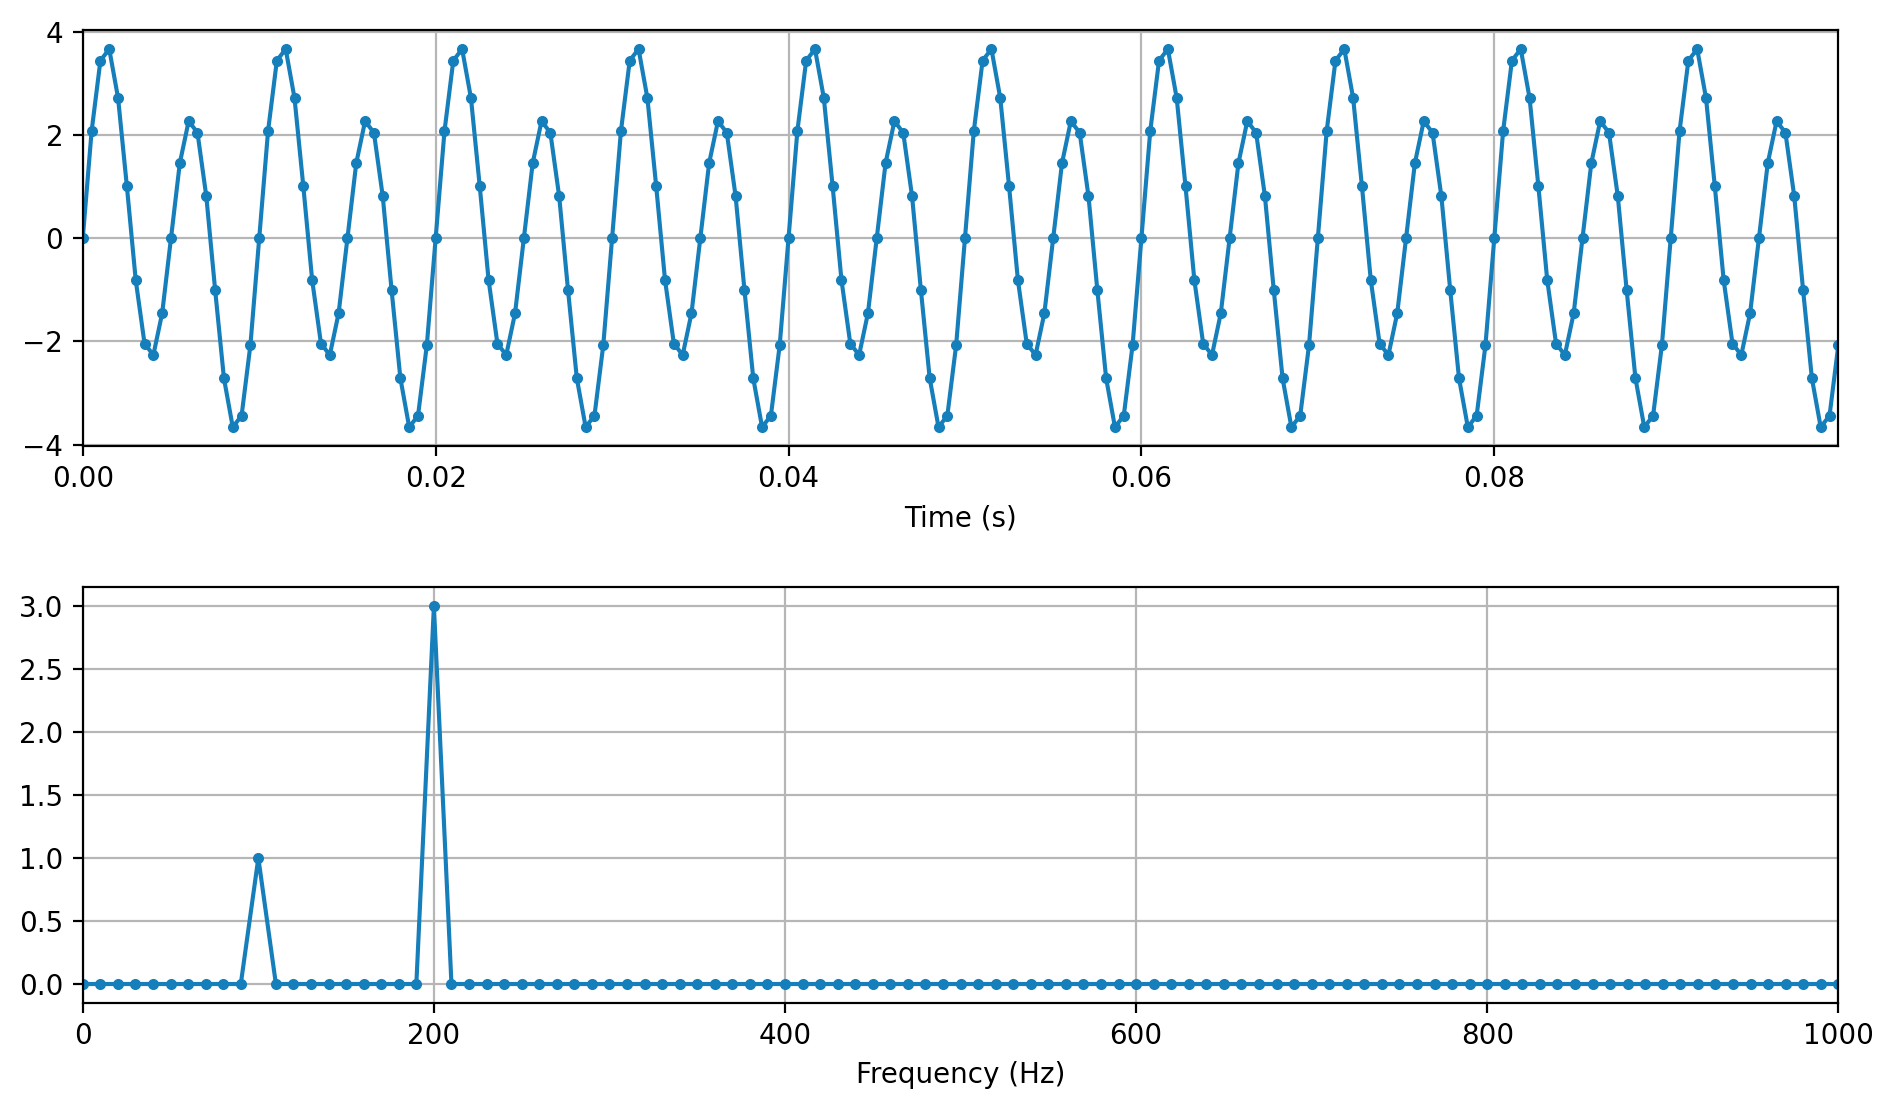
\includegraphics[width=16cm]{TimeDomain to FreqDomain fft.png}
%    \caption{Matplotlib graph of FT taking Time to Frequency domain \parencite{GitHubRepo}}
%\end{figure}

%Listings of code
\newpage
\lstinputlisting[language = Python, style = chstyle, caption = main.py]{main.py}
\lstinputlisting[language = Python, style = chstyle, caption = compute.py]{compute.py}
\lstinputlisting[language = Python, style = chstyle, caption = webscrape.py]{webscrape.py}

\newpage
\lstinputlisting[language = Python, style = chstyle, caption = Fourier Transform Demonstration]{FourierTransformDemo.py}
\begin{figure}[h!]
    \centering
    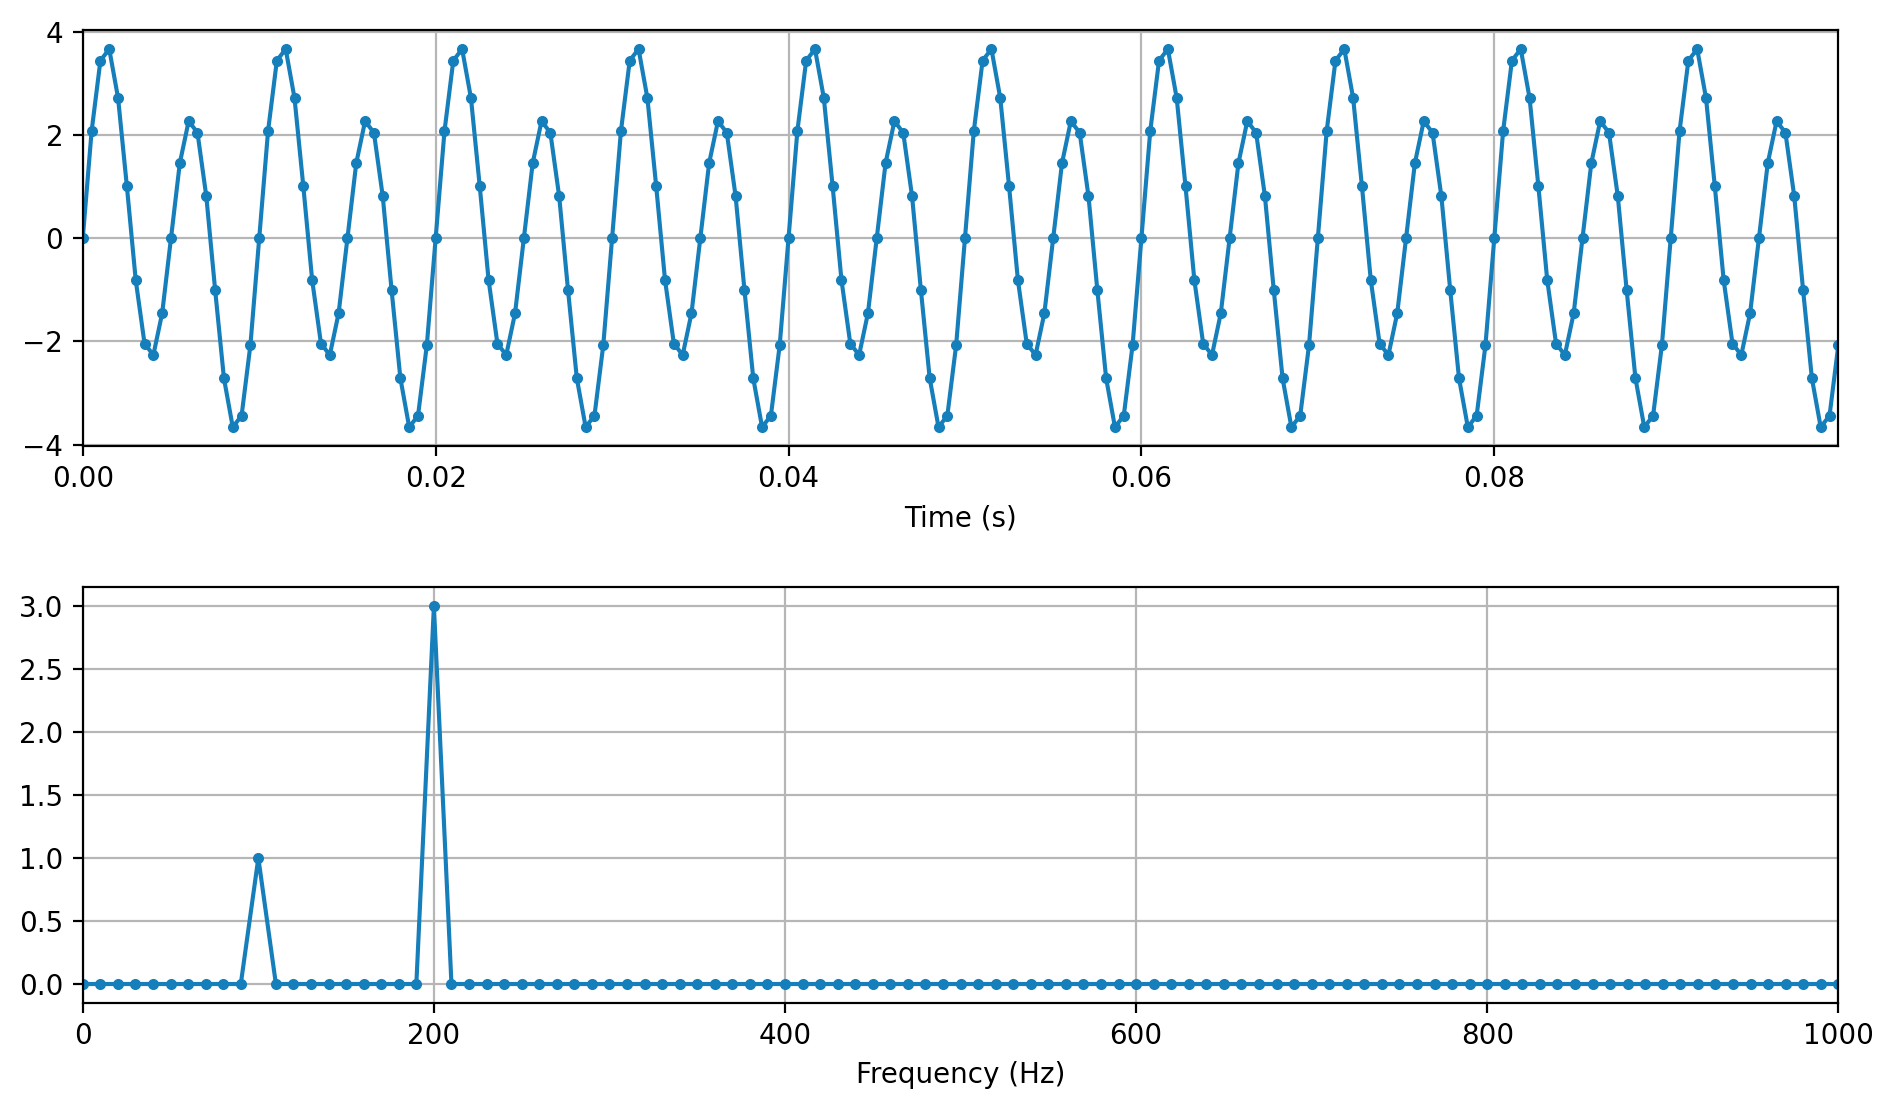
\includegraphics[width=16cm]{FourierTransform Demo.png}
    \caption{Matplotlib graph of FT taking Time to Frequency domain \parencite{GitHubRepo}}
\end{figure}

\section{Postface}
This project was incredibly useful in exposing me to the mathematics behind many first year EEE/ EIE degrees. Along the way I gained a lot of practical techincal information in python,
such as Object-Oriented Programming, file-handling and proficiency with multiple libraries. This let me perform a wide range of objectives from data analysis, web-scraping to using logic to come to a solution.
With more time, I would have looked to either Tkinter or web-development to be able to host my application on a more User-Friendly level (and hope to come back to this later). 
I also learnt how to host software on GitHub, intricacies on VSCode IDE, and also LaTeX. Audio Signal Processing is a much broader topic than what hasa been covered, and I look forward to returning to it.

\newpage
%Bibliography
\section{Bibliography}
\doublespacing
\printbibliography[heading = none]

\end{document}   